\chapter{线性代数中的线性方程组}
\section{线性方程组}
线性方程:
	\[ a_{1}x_{1}+a_{2}x_{2}+\cdots +a_{n}x_{n}=b \]
其中, $b$与系数$a_{1}$,$a_{2}$,$\cdots$,$a_{n}$是实数或复数, 通常为已知数. n为任意正整数\\[2ex]

线性方程组 -- 由一个或几个包含相同变量的线性方程组成, 如:
\[\left\{\begin{array}{r@{\hspace{1.5pt}}l@{\hspace{1.5pt}}r@{\hspace{1.5pt}}l@{\hspace{1.5pt}}r@{\hspace{1.5pt}}l@{\hspace{1.5pt}}r}
	2x_1 & - & x_2 & + & 1.5x_3 & = & 8\\
	x_1  &   &     & - & 4x_3   & = & -7		
\end{array}\right.\]
若线性方程组的方程个数少于未知数个数, 称之为\textbf{欠定方程组}\\
若线性方程组的方程个数多余未知数个数, 称之为\textbf{超定方程组}\\
方程组所有可能的解的集合称为线性方程组的\textbf{解集}\\
若两个方程组有相同的解集, 则这两个方程组称为\textbf{等价}的\\[2ex]

线性方程组解集情况:\\
1.无解;\\
2.有唯一解;\\
3.有无穷多解.\\[1ex]
当方程组无解时, 称线性方程组\textbf{不相容}\\
当方程组有唯一解或无穷多解时, 称线性方程组\textbf{相容}\\[2ex]

线性方程组
\[\left\{\begin{array}{r@{\hspace{1.5pt}}l@{\hspace{1.5pt}}r@{\hspace{1.5pt}}l@{\hspace{1.5pt}}r@{\hspace{1.5pt}}l@{\hspace{1.5pt}}r}
x_1 & - & 2x_2 & + &  x_3 & = & 0\\
	& 	& 2x_2 & - & 8x_3 & = & 8\\
-4x_1 & + & 5x_2 & + & 9x_3 & = & -9
\end{array}\right.\]
线性方程组的\textbf{系数矩阵}
\[\left[\begin{array}{r r r}
	1 & -2 & 1\\
	0 & 2  & -8\\
	-4 & 5 & 9
\end{array}\right]\]
线性方程组的\textbf{增广矩阵}
\[\left[\begin{array}{r r r r}
	1 & -2 & 1 & 0\\
	0 & 2  & -8 & 8\\
	-4 & 5 & 9 & -9
\end{array}\right]\]\\[2ex]

解线性方程组\\
思路: 将方程组用一个更容易求解的等价方程组替代\\

化简方程组的三种基本变换:\\
1.倍加变换 - 将某方程替换为它与另一方程倍数的和;\\
2.对换变换 - 交换两个方程的位置;\\
3.倍乘变换 - 方程的所有系数乘以一个非0实数.\\

例. 简化如下方程组
\[\begin{array}{r@{\hspace{1.5pt}}l@{\hspace{1.5pt}}r@{\hspace{1.5pt}}l@{\hspace{1.5pt}}r@{\hspace{1.5pt}}l@{\hspace{1.5pt}}r}
x_1 & - & 2x_2 & + &  x_3 & = & 0\\
	& 	& 2x_2 & - & 8x_3 & = & 8\\
-4x_1 & + & 5x_2 & + & 9x_3 & = & -9
\end{array}\qquad\left[\begin{array}{r r r r}
	1 & -2 & 1 & 0\\
	0 & 2 & -8 & 8\\
	-4 & 5 & 9 & -9
\end{array}\right]\]
步骤1 -- \ding{194}+4\ding{192}
\[\left[\begin{array}{r r r r}
    1 & -2 & 1 & 0\\
    0 & 2 & -8 & 8\\
    -4 & 5 & 9 & -9
\end{array}\right] \Rightarrow \left[\begin{array}{r r r r}
    1 & -2 & 1 & 0\\
    0 & 2 & -8 & 8\\
    0 & -3 & 13 & -9
\end{array}\right]\]
步骤2 -- $\dfrac{1}{2}$\ding{193}
\[\left[\begin{array}{r r r r}
    1 & -2 & 1 & 0\\
    0 & 2 & -8 & 8\\
    0 & -3 & 13 & -9
\end{array}\right] \Rightarrow \left[\begin{array}{r r r r}
    1 & -2 & 1 & 0\\
    0 & 1 & -4 & 4\\
    0 & -3 & 13 & -9
\end{array}\right]\]
步骤3 -- \ding{194}+3\ding{193}
\[\left[\begin{array}{r r r r}
    1 & -2 & 1 & 0\\
    0 & 1 & -4 & 4\\
    0 & -3 & 13 & -9
\end{array}\right] \Longrightarrow \left[\begin{array}{r r r r}
	1 & -2 & 1 & 0\\
	0 & 1 & -4 & 4\\
	0 & 0 & 1 & 3
\end{array}\right]\]
步骤4 -- \ding{193}+4\ding{194}
\[\left[\begin{array}{r r r r}
    1 & -2 & 1 & 0\\
    0 & 1 & -4 & 4\\
    0 & 0 & 1 & 3
\end{array}\right] \Longrightarrow \left[\begin{array}{r r r r}
	1 & -2 & 1 & 0\\
	0 & 1 & 0 & 16\\
	0 & 0 & 1 & 3
\end{array}\right]\]
步骤5 -- \ding{192}+(-\ding{194})
\[\left[\begin{array}{r r r r}
    1 & -2 & 1 & 0\\
    0 & 1 & 0 & 16\\
    0 & 0 & 1 & 3
\end{array}\right] \Longrightarrow \left[\begin{array}{r r r r}
	1 & -2 & 0 & -3\\
	0 & 1 & 0 & 16\\
	0 & 0 & 1 & 3
\end{array}\right]\]
步骤6 -- \ding{192}+2\ding{193}
\[\left[\begin{array}{r r r r}
    1 & -2 & 0 & -3\\
    0 & 1 & 0 & 16\\
    0 & 0 & 1 & 3
\end{array}\right] \Longrightarrow \left[\begin{array}{r r r r}
	1 & 0 & 0 & 29\\
	0 & 1 & 0 & 16\\
	0 & 0 & 1 & 3
\end{array}\right]\]
\framebox{若两个线性方程组的增广矩阵是行等价的, 则它们具有相同的解集}\vspace{6ex}

\section{行化简与阶梯形矩阵}
非零行(列): 矩阵中至少包含一个非零元素的行(列)\\
先导元素: 该行最左边的非零元素\\
\begin{definition}
一个矩阵称为阶梯形, 若它有以下三个性质:\\
1.所有非零行在零行之上;\\
2.某一行先导元素的列位于上一行先导元素的右边;\\
3.某一先导元素所在列下方元素都是零;\\
若还满足以下性质, 则称为简化阶梯形:\\
4.每一非零行的先导元素是1;\\
5.每一先导元素是该元素所在列的唯一非零元素.
\end{definition}\vspace{2ex}

\begin{TheoremTwo}[简化阶梯形矩阵的唯一性]
每个矩阵行等价于唯一的简化阶梯形矩阵.
\end{TheoremTwo}\vspace{2ex}

\begin{definition}
矩阵A中的{\heiti 主元位置}是A中对应于它的阶梯形中先导元素的位置.{\heiti 主元列}是A中含有主元位置的列.
\end{definition}\vspace{2ex}

基本变量: 位于主元列的变量\\
自由变量: 位于非主元列的变量\\[2ex]

\begin{TheoremTwo}[存在与唯一性定理]
线性方程组相容的充要条件是增广矩阵的最右列不是主元列. 也就是说, 增广矩阵的阶梯形没有形如
	\[[0\ \cdots\ 0\ b], b\neq 0\]
的行. 若线性方程组相容, 则它的解集可能有两种情形:\\
1)当没有自由变量时, 有唯一解;\\
2)若至少有一个自由变量, 则有无穷多解.
\end{TheoremTwo}\vspace{2ex}

应用行化简算法解线性方程组:\\
1.写出方程组的增广矩阵\\
2.应用行化简算法把增广矩阵化为阶梯形, 确定方程组是否相容, 如果没有解则停止; 否则进行下一步\\
3.继续行化简算法得到它的简化阶梯形\\
4.写出简化阶梯形矩阵对应的方程组\\
5.将每个非零方程改写为使用自由变量表示基本变量的形式\\[4ex]

\section{向量方程}
列向量: 仅含一列的矩阵, 简称为向量. 如:
\[u=\left[\begin{array}{c}
	3\\
	-1
\end{array}\right] \text{\quad or\quad} u=(3, -1)\]\\[2ex]
行向量: 仅含一行的矩阵. 如:
\[v=\left[\begin{array}{c c}
	2 & 5
\end{array}\right]\]\\[2ex]
所有两个元素的向量表示为$\mathbb{R}^2$, $\mathbb{R}$表示元素为实数, 2表示向量包含两个元素\\
向量加法:
\begin{equation*}
\left[\begin{array}{c}
	1\\
	-2
\end{array}\right]
+
\left[\begin{array}{c}
	2\\
	5
\end{array}\right]
=
\left[\begin{array}{c}
	1+2\\
	-2+5
\end{array}\right]
=
\left[\begin{array}{c}
	3\\
	3
\end{array}\right]
\end{equation*}
标量乘法:\\
\indent 若$u=\left[\begin{array}{c}3\\-1\end{array}\right]$, $c=5$, 则:
\[cu=5\left[\begin{array}{c}3\\-1\end{array}\right]=\left[\begin{array}{c}15\\-5\end{array}\right]\]

向量$\left[\begin{array}{r}x\\y\end{array}\right]$的几何含义: 由原点(0,0)指向点(x,y)的有向线段\\[2ex]

\begin{law}[向量加法的平行四边形法则]\ \\
若$\mathbb{R}^2$中向量$\mathbf{u}$和$\mathbf{v}$用平面上的点表示, 则$\mathbf{u+v}$对应于以$\mathbf{u}$,$\mathbf{0}$和$\mathbf{v}$为三个顶点的平行四边形的第4个顶点, 如图.\\[2ex]
\begin{center}
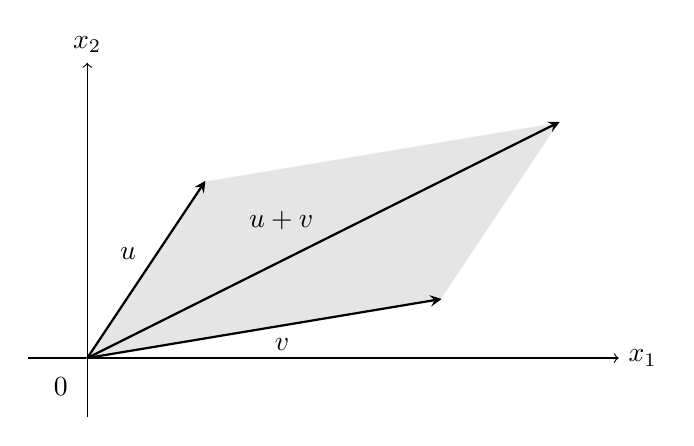
\begin{tikzpicture}[scale=0.75]
\draw[->] (-1,0) -- (9,0) node[right]{$x_1$};
\draw[->] (0,-1) -- (0,5) node[above]{$x_2$};
\draw[color=white, fill=black!10] (0,0) -- (6,1) -- (8,4) -- (2,3) -- cycle;
\draw[-stealth, thick, auto] (0,0) -- (2,3) node[pos=0.5]{$u$};
\draw[-stealth, thick, auto, swap] (0,0) -- (6,1) node[pos=0.5]{$v$};
\draw[-stealth, thick, auto] (0,0) -- (8,4) node[pos=0.5]{$u+v$};
\node at (0,0) [label=below left:$0$]{};
\end{tikzpicture}
\end{center}
\end{law}\vspace{3ex}

所有元素都是零的向量称为\textbf{零向量}, 用\textbf{0}表示(\textbf{0}中元素的个数可由上下文确定)\\[2ex]

\begin{law}[$\mathbb{R}^n$中向量的代数性质]\ \\
对$\mathbb{R}^n$中一切向量$\mathbf{u}$,$\mathbf{v}$,$\mathbf{w}$以及标量$c$和$d$:
\begin{equation*}
\begin{array}{l@{}c@{}l l l@{}c@{}l l}
( & i & ) & \mathbf{u}+\mathbf{v}=\mathbf{v}+\mathbf{u} & ( & v & ) & c(\mathbf{u}+\mathbf{v})=c\mathbf{u}+c\mathbf{v}\\
( & ii & ) & (\mathbf{u}+\mathbf{v})+\mathbf{w}=\mathbf{u}+(\mathbf{v}+\mathbf{w}) & ( & vi & ) & (c+d)\mathbf{u}=c\mathbf{u}+d\mathbf{u}\\
( & iii & ) & \mathbf{u}+\mathbf{0}=\mathbf{0}+\mathbf{u}=\mathbf{u} & ( & vii & ) & c(d\mathbf{u})=(cd)\mathbf{u}\\
( & iv & ) & \mathbf{u}+(-\mathbf{u})=-\mathbf{u}+\mathbf{u}=\mathbf{0} & ( & viii & ) & 1\mathbf{u}=\mathbf{u}
\end{array}
\end{equation*}
\end{law}\vspace{2ex}

给定$\mathbb{R}^n$中向量$\mathbf{v}_1$,$\mathbf{v}_2$,$\cdots$,$\mathbf{v}_p$和标量$c_1$,$c_2$,$\cdots$,$c_p$, 向量
	\[\mathbf{y}=c_1\mathbf{v}_1+\cdots+c_p\mathbf{v}_p\]
称为向量$\mathbf{v}_1$,$\mathbf{v}_2$,$\cdots$,$\mathbf{v}_p$以$c_1$,$c_2$,$\cdots$,$c_p$为\textbf{权}的\textbf{线性组合}.\\[2ex]

\framebox{
\begin{minipage}{\linewidth}
向量方程
\[x_1\mathbf{a}_1+x_2\mathbf{a}_a+\cdots+x_n\mathbf{a}_n=\mathbf{b}\]
和增广矩阵为
\begin{equation}
[\mathbf{a}_1\quad\mathbf{a}_2\quad\cdots\quad\mathbf{a}_n\quad\mathbf{b}]\label{matrix:eq_01}
\end{equation}
的线性方程组有相同的解集. 特别地, $\mathbf{b}$可表示为$\mathbf{a}_1$,$\mathbf{a}_2$,$\cdots$,$\mathbf{a}_n$的线性组合当且仅当对应于\eqref{matrix:eq_01}式的线性方程组有解.
\end{minipage}}\\[4ex]

\begin{definition}
若$\mathbf{v}_1$,$\mathbf{v}_2$,$\cdots$,$\mathbf{v}_p$是$\mathbb{R}^n$中的向量, 则$\mathbf{v}_1$,$\mathbf{v}_2$,$\cdots$,$\mathbf{v}_p$的所有线性组合所成的组合用记号$\Span\{\mathbf{v}_1$,$\mathbf{v}_2$,$\cdots$,$\mathbf{v}_p\}$表示, 称为由$\mathbf{v}_1$,$\mathbf{v}_2$,$\cdots$,$\mathbf{v}_p$所\textbf{生成}(或\textbf{张成})\textbf{的$\mathbb{R}^n$的子集}. 也就是说, $\Span\{\mathbf{v}_1$,$\mathbf{v}_2$,$\cdots$,$\mathbf{v}_p\}$是所有形如
	\[c_1\mathbf{v}_1+c_2\mathbf{v}_2+\cdots+c_p\mathbf{v}_p\]
的向量的集合, 其中$c_1$,$c_2$,$\cdots$,$c_p$为标量.\\[2ex]
\end{definition}\vspace{4ex}

\section{矩阵方程$A\mathbf{x}=\mathbf{b}$}
\begin{definition}
若$A$是$m\times n$矩阵, 它的各列为$\bm{a}_1$,$\cdots$,$\bm{a}_n$. 若$\bm{x}$是$\mathbb{R}^n$中的向量, 则\textbf{$A$与$\bm{x}$的积}(记为$A\bm{x}$)就是\textbf{$A$的各列以$\bm{x}$中对应元素为权的线性组合}, 即
	\[A\bm{x}=[\bm{a}_1\ \bm{a}_2\ \cdots\ \bm{a}_n]\left[\begin{array}{c}x_1\\x_2\\\vdots\\x_n\end{array}\right]=x_1\bm{a}_1+x_2\bm{a}_2+\cdots+x_n\bm{a}_n\]
注意$A\bm{x}$仅当$A$的列数等于$\bm{x}$中的元素个数时才有意义.\\[2ex]
\end{definition}

\begin{TheoremOne}
若$A$是$m\times n$矩阵, 它的各列为$\bm{a}_1$,$\cdots$,$\bm{a}_n$, 而$\bm{b}$属于$\mathbb{R}^n$, 则矩阵方程
\[A\bm{x}=\bm{b}\]
与向量方程
\[x_1\bm{a}_1+x_2\bm{a}_2+\cdots+x_n\bm{a}_n=\bm{b}\]
有相同的解集. 它又与增广矩阵为
\[[\bm{a}_1\ \bm{a}_2\ \cdots\ \bm{a}_n\ \bm{b}]\]
的线性方程组有相同的解集.\\[2ex]
\end{TheoremOne}\vspace{2ex}

\begin{TheoremOne}
设$A$是$m\times n$矩阵, 则下列命题是逻辑上等价的. 也就是说, 对某个$A$, 它们都成立或者都不成立.\\
\begin{tabular}{l@{\,}l}
a. & 对$\mathbb{R}^m$中每个$\bm{b}$, 方程$A\bm{x}=\bm{b}$有解.\\
b. & $\mathbb{R}^m$中的每个$\bm{b}$都是$A$的列的一个线性组合.\\
c. & $A$的各列生成$\mathbb{R}^m$.\\
d. & $A$在每一行都有一个主元位置.\\[2ex]
\end{tabular}
\end{TheoremOne}\vspace{2ex}

\begin{law}[计算$A\bm{x}$的行---向量规则]\ \\
若乘积$A\bm{x}$有定义, 则$A\bm{x}$中的第$i$个元素是$A$的第$i$行元素与$\bm{x}$的相应元素乘积之和.
\end{law}\vspace{2ex}

矩阵的主对角线上元素为1, 其他位置上元素为0, 这个矩阵称为\textbf{单位矩阵}, 并记为$I$.\\
如果矩阵为$n\times n$单位矩阵, 记为$I_n$.\\[2ex]

\begin{TheoremOne}
若$A$是$m\times n$矩阵, $\bm{u}$和$\bm{v}$是$\mathbb{R}^n$中向量, c是标量, 则\\
\begin{tabular}{l@{\,}l}
a. & $A(\bm{u}+\bm{v})=A\bm{u}+A\bm{v}$\\
b. & $A(c\bm{u})=c(A\bm{u})$
\end{tabular}
\end{TheoremOne}\vspace{6ex}

\section{线性方程组的解集}
若线性方程组可写成
\[A\bm{x}=\bm{0}\]
的形式, 则称为\textbf{齐次线性方程组}. 其中, $A$是$m\times n$矩阵, $\bm{0}$是$\mathbb{R}^m$中的零向量.\\
齐次线性方程组至少有一个解, 即$\bm{x}=\bm{0}$($\mathbb{R}^n$中的零向量), 这个解称为它的\textbf{平凡解}.\\
如果有一个非零向量$\bm{x}$, 满足$A\bm{x}=\bm{0}$, 这个解称为它的\textbf{非平凡解}.\\[2ex]

\begin{law}
齐次方程$A\bm{x}=\bm{0}$有非平凡解当且仅当方程至少有一个自由变量.
\end{law}\vspace{2ex}

$\bm{x}=s\bm{u}+t\bm{v}$为$A\bm{x}=\bm{0}$的\textbf{参数向量形式}, 并称之为\textbf{参数向量方程}. 其中, $s$,$t$为自由变量\\
$\bm{x}=\bm{p}+t\bm{v}$为$A\bm{x}=\bm{b}$的\textbf{参数向量形式}, 并称之为\textbf{参数向量方程}. 其中, $t$为自由变量\\
例.\\
$x_1=0.3x_2+0.2x_3$\\[1ex]
$\bm{x}=
\left[\begin{array}{l}
x_1\\
x_2\\
x_3
\end{array}\right]=
\left[\begin{array}{c}
0.3x_2+0.2x_3\\
x_2\\
x_3
\end{array}\right]=
\left[\begin{array}{r}
0.3x_2\\
x_2\\
0
\end{array}\right]+\left[\begin{array}{r}
0.2x_3\\
0\\
x_3
\end{array}\right]\\
\phantom{\bm{x}}=x_2\left[\begin{array}{r}
0.3\\
1\\
0
\end{array}\right]+x_3\left[\begin{array}{r}
0.2\\
0\\
1
\end{array}\right]
$\\[1ex]
因此, $A\bm{x}=\bm{b}$的解集是一条通过$\bm{p}$而平行于$A\bm{x}=\bm{0}$的解集的直线. 也称为将$\bm{v}$沿着$\bm{p}$进行直线移动.\\[2ex]

\begin{TheoremOne}
设方程$A\bm{x}=\bm{b}$对某个$\bm{b}$是相容的, $\bm{p}$为一个特解, 则$A\bm{x}=\bm{b}$的解集是所有形如$\bm{w}=\bm{p}+\bm{v}_h$的向量的集, 其中$\bm{v}_h$时齐次方程$A\bm{x}=\bm{b}$的任意一个解.
\end{TheoremOne}\vspace{3ex}

\begin{law}[把(相容方程组的)解集表示成参数向量形式]\ \\
1.把增广矩阵简化为简化阶梯形.\\
2.把每个基本变量用自由变量表示.\\
3.把一般解$\bm{x}$表示成向量, 如果有自由变量, 其元素依赖于自由变量.\\
4.把$\bm{x}$分解为向量(元素为常数)的线性组合, 用自由变量作为参数.
\end{law}\vspace{4ex}

\section{线性方程组的应用}
1.经济学 - 部分的收支平衡\\
2.化学式 - 等号两边原子守恒\\
3.网络流 - 节点的进/出流量恒等\\[4ex]

\section{线性无关}
\begin{definition}
$\mathbb{R}^n$中一组向量$\{\bm{v}_1$,$\cdots$,$\bm{v}_p\}$称为\textbf{线性无关}的, 若向量方程
\[x_1\bm{v}_1+x_2\bm{v}_2+\cdots+x_p\bm{v}_p=\bm{0}\]
仅有平凡解. 向量组(集)$\{\bm{v}_1$,$\cdots$,$\bm{v}_p\}$称为\textbf{线性相关}的, 若存在不全为零的权$c_1$,$\cdots$,$c_p$, 使
\[c_1\bm{v}_1+c_2\bm{v}_2+\cdots+c_p\bm{v}_p=\bm{0}\]
\end{definition}\vspace{2ex}

\begin{law}
矩阵$A$的各列线性无关, 当且仅当方程$A\bm{x}=\bm{0}$仅有平凡解.
\end{law}\vspace{2ex}

\begin{law}
两个向量的集合$\{\bm{v}_1$,$\bm{v}_2\}$线性相关, 当且仅当其中一个向量是另一个向量的倍数. 这个集合线性无关, 当且仅当其中任一个向量都不是另一个向量的倍数.
\end{law}\vspace{4ex}

\begin{TheoremTwo}[线性相关集的特征]
两个或更多个向量的集合$S=\{\bm{v}_1,\cdots,\bm{v}_p\}$线性相关, 当且仅当S中至少有一个向量是其他向量的线性组合. 事实上, 若S线性相关, 且$\bm{v}_1\neq\bm{0}$, 则某个$\bm{v}_j$$(j>1)$是它前面向量$\bm{v}_1$,$\cdots$,$\bm{v}_{j-1}$的线性组合.
\end{TheoremTwo}\vspace{4ex}

\begin{TheoremOne}
若一个向量组的向量个数超过每个向量的元素个数, 那么这个向量组线性相关. 就是说, $\mathbb{R}^n$中任意向量组$\{\bm{v}_1$,$\cdots$,$\bm{v}_p\}$当$p>n$时线性相关.
\end{TheoremOne}\vspace{4ex}

\begin{TheoremOne}
若$\mathbb{R}^n$中向量组$S=\{\bm{v}_1,\cdots,\bm{v}_p\}$包含零向量, 则它线性相关.
\end{TheoremOne}\vspace{4ex}

\section{线性变换介绍}
由$\bm{x}$到$A\bm{x}$的对应是由一个向量集到另一个向量集的函数\\[2ex]

\begin{definition}
变换(或映射)$T$称为\textbf{线性}的, 若\\
\begin{tabular}{l@{}c@{}l@{\hspace{2pt}}l}
$($ & i & $)$ & 对$T$的定义域中一切$\bm{u}$,$\bm{v}$,$T(\bm{u}+\bm{v})=T(\bm{u})+T(\bm{v})$.\\
$($ & ii & $)$ & 对$T$的定义域中的一切$\bm{u}$和数$c$, $T(c\bm{u})=cT(\bm{u})$.
\end{tabular}
\end{definition}\vspace{4ex}

\begin{law}
若T是线性变换, 则
\[T(\bm{0})=\bm{0}\]
且对$T$的定义域中一切向量$\bm{u}$和$\bm{v}$以及数$c$和$d$, 有:
\[T(c\bm{u}+d\bm{v})=cT(\bm{u})+dT(\bm{v})\]
\end{law}\vspace{6ex}

\section{线性变换的矩阵}
\begin{TheoremOne}
设$T$:$\mathbb{R}^n\rightarrow\mathbb{R}^m$为线性变换, 则存在唯一的矩阵$A$, 使得对$\mathbb{R}^n$中一切$\bm{x}$, 有
\[T(\bm{x})=A\bm{x}\]
事实上, $A$是$m\times n$矩阵, 它的第$j$列是向量$T(\bm{e}_j)$, 其中$\bm{e}_j$是$\mathbb{R}^n$中单位矩阵$\bm{I}_n$的第$j$列:
\[A=[T(\bm{e}_1)\ \cdots\ T(\bm{e}_n)]\]
\end{TheoremOne}\vspace{4ex}

\begin{definition}
映射$T$:$\mathbb{R}^n\rightarrow\mathbb{R}^m$称为到$\mathbb{R}^m$上的映射, 若$\mathbb{R}^m$中每个$\bm{b}$是$\mathbb{R}^n$中至少一个$\bm{x}$的像(也称为\textbf{满射}).
\end{definition}\vspace{4ex}

\begin{definition}
映射$T$:$\mathbb{R}^n\rightarrow\mathbb{R}^m$称为\textbf{一对一映射}(或1:1), 若$\mathbb{R}^m$中每个$\bm{b}$是$\mathbb{R}^n$中至多一个$\bm{x}$的像(也称为\text{单射}).
\end{definition}\vspace{4ex}

\begin{TheoremOne}
设$T$:$\mathbb{R}^n\rightarrow\mathbb{R}^m$为线性变换, 则$T$是一对一的当且仅当方程$A\bm{x}=\bm{0}$仅有平凡解.
\end{TheoremOne}\vspace{4ex}

\begin{TheoremOne}
设$T$:$\mathbb{R}^n\rightarrow\mathbb{R}^m$是线性变换, 设$A$为$T$的标准矩阵, 则\\
\begin{tabular}{l@{\ }l}
a. & $T$把$\mathbb{R}^n$映上到$\mathbb{R}^m$, 当且仅当$A$的列生成$\mathbb{R}^m$.\\
b. & $T$是一对一的, 当且仅当$A$的列线性无关.
\end{tabular}
\end{TheoremOne}\vspace{6ex}

\section{商业、科学和工程中的线性模型}
\begin{law}[基尔霍夫电压定律]\ \\
围绕一条回路同一方向的电压降$RI$的代数和等于围绕该回路的同一方向电动势的代数和.
\end{law}\vspace{4ex}

\begin{law}
如果有矩阵$A$使$\bm{x}_1=A\bm{x}_0$,$\bm{x}_2=A\bm{x}_1$, 一般地,
\[\bm{x}_{k+1}=A\bm{x}_k\text{,\ }k=0,1,2,\cdots\]
则称为\textbf{线性差分方程}(或\textbf{递归关系}).
\end{law}
